\documentclass[12pt,swedish]{article}

% Språk
\usepackage[swedish]{babel}
\usepackage[utf8]{inputenc}
\usepackage{titling}
\usepackage{listings}

% Tabell och diagram
\usepackage{booktabs}
\usepackage{float}

% Bilder
\usepackage{graphicx}
\graphicspath{{images/}}

% Referenser
\usepackage[style=authoryear,backend=biber,texencoding=utf8,bibencoding=utf8,natbib]{biblatex}
\usepackage{csquotes}
\addbibresource{bibliography.bib}

% Lägg till ytterligare titeldata
\postauthor{\end{tabular}\par jnikl@kth.se \par Grupp B:6\end{center}}

% Titeldata
\title{Finns det samband mellan ett programspråks ålder och dess beräkningshastighet?}
\author{Johan Niklasson}
\date{2017-11-20}

% Öppna dokumentet
\begin{document}
% Så det inte blir någon sidnumrering sker på första sidan
\pagenumbering{gobble}

% Titelsida
\maketitle
\normalsize
\begin{center}

\begin{abstract}
Kan programspråk som lanserades för 45 år sedan vara snabbare än programspråk som lanseras idag? För att undersöka detta gjordes experiment på sex olika kompilerade programspråk med ett spann på 37 år mellan det äldsta och yngsta. Mätningarna gjordes med algoritmen Collatz problem, som programmerades i de olika språken och sedan kördes på en Raspberry Pi för att uppmäta hur lång tid varje programspråk tog på sig att lösa problemet. Studien visade att programspråken faktiskt har blivit snabbare med tiden, trots att vissa teorier motsätter sig resultatet.
\end{abstract}
\end{center}
\clearpage

% Börja sidnumreringen
\pagenumbering{arabic}

% Innehållsförteckning
\tableofcontents
\clearpage


\section{Inledning}
Ett programspråk är en formell och strikt uppsättning av instruktioner som en dator kan läsa för att utföra uppgifter. Sedan det första programspråket utvecklades i elektroniska komponenter år 1945 \citep{bauer_wossner_1972} har det lanserats flera hundra nya programspråk. Vissa programspråk utvecklas för att lösa specifika problem - programspråket Erlang av Ericsson som exempel skapades för styrsystemen i telefonväxlar \citep{armstrong_1997}. Andra språk, såsom Scratch, har tagits fram i undervisningssyfte för barn \citep{maloney_resnick_rusk_silverman_eastmond_2010}.

Men även då vissa programspråk har haft vissa typer av uppgifter i hänsyn vid sin framtagning, har dessa då samtidigt lyckats bli snabbare? Moores Lag som beskriver att antalet transistorer på chip växer potentiellt, resulterar i datorer och processorer blir snabbare varje år \citep{schaller_1997}. Kan det därför finnas ett mindre behov av att nyare programspråk inte behöver vara lika snabba utan kanske istället till exempel mer lättlästa för människor?

\subsection{Syfte}
Syftet med studien är att ta fram ett underlag om varför nya programspråk lanseras. Då det kan vara flera egenskaper som påverkar framtagningen och användningen av programspråk har ett fokus koncentrerats på en av dessa - beräkningshastigheten hos ett programspråk.

\subsection{Frågeställning}
Frågeställningen för studien är: “Finns det någon korrelation i beräkningshastighet och utgivningsår för kompilerade mellannivåspråk?”

\subsection{Avgränsning}
I studien är det endast intressant att jämföra språk med liknande egenskaper. Därför kommer endast kompilerbara mellannivåspråk att testas som går att exekveras (köras) och kompileras på en Raspberry Pi (en liten enkortsdator i storleken av ett kreditkort) i operativsystemet Raspbian.


\section{Begrepp}
I studien används ett antal termer som är relevanta för experimentet. I detta avsnitt kommer dessa förklaras förenklade för att underlätta vad de innebär.

\subsection{Programkod}
En programkod är en uppsättning instruktioner som utförs av en dators processor. Instruktionerna består av jämförelser eller matematiska operationer av två värden som sedan utför efterföljande instruktioner beroende på resultatet.

\subsection{Processor}
Processorn brukar hänvisas som “hjärnan” i en dator som utför de flesta av instruktionerna från en programkod \citep{charuba_1996}. Den här studien kommer enbart fokusera på tiden för de beräkningar som processorn utför.

\subsection{Kompilering}
Att kompilera en programkod innebär att programkoden skrivs om från beskrivande syntaxer till maskinkod som processorn kan läsa. I programmeringsspråk brukar en så kallad IF-sats, som kontrollerar villkor, skrivas som följande:
\begin{lstlisting}
IF condition THEN
    sequence 1
ELSE
    sequence 2
ENDIF
\end{lstlisting}
Detta är inte programkod som processorn kan tolka utan måste först skrivas om till instruktioner den kan förstå. Denna omskrivning kallas för kompilering. Ett program som kallas för kompilator gör just detta och skriver om den programkoden till det förväntade formatet, så kallad maskinkod \citep{srikant_shankar_2008}.

\subsection{Nivåer på programspråk}
Inom programmering är det skillnad på hur programspråk fungerar på enheten de körs. I studien kommer endast mellannivåspråk att användas.
\begin{description}
    \item [Mellannivåspråk:] I ett mellannivåspråk kompileras programkoden innan den exekveras. Det kan liknas med att samtliga läses en gång och utförs sedan direkt efter varandra utan att behöva läsa om dem.
    \item [Högnivåspråk:] Ett högnivåspråk kompilerar programkoden samtidigt som instruktionerna utförs. Det innebär att varje instruktion läses precis innan den utförs och resulterar därför i att programkoden exekveras långsammare än i ett mellannivåspråk \citep{maclachlan_1992}.
\end{description}

\subsection{Collatz problem}
Collatz problem är ett olöst matematiskt problem inom talteorin. Problemet beskriver ett sätt utföra ett antal matematiska instruktioner i följd efter varandra för att nå ett sluttal. Instruktionerna är följande:
\begin{enumerate}
    \item [1.] Välj ett positivt heltal \( n \) som är större än ett.
    \item [2.] Om \( n \) är jämnt, dividera det med två. Om \( n \) är udda, multiplicera det med tre och addera ett.
    \item [3.] Repetera steg två tills \( n \) når ett.
\end{enumerate}
I studien kommer detta problem skrivas om till en algoritm som utför stegen ovan för enskilda tal. Algoritmen används sedan för att utföra instruktioner som då går att mäta mot varandra i olika programspråk. Algoritmen använder endast addition, multiplikation, division och modulo (för att se om ett tal är jämnt eller udda) som matematiska operationer.

Algoritmen är oförutsägbar för olika tal då det inte finns något mönster för hur många iterationer den kräver innan talet når ett. Detta har dock ingen inverkan i jämförelser mellan olika programspråk så länge samma tal jämförs, eftersom samma tal alltid genererar samma antal steg. 


\newpage
\section{Metod}
Ett initialt urval på programspråk gjordes utifrån de mest använda programspråken idag från \citeauthor{tiobe} (\citeyear{tiobe}). Detta gjordes för det skulle finnas en relevans till användning av de språk som ingick i studien. Av dessa 25 var det cirka hälften som var mellannivåspråk och ytterligare en halvering skedde efter att ha filtrerat bort de språk som inte var kompatibla på en Raspberry Pi. Språken med sina respektive utgivningsår som återstod blev då följande:

\begin{itemize}
    \item C (1972)
    \item Ada (1980)
    \item C++ (1983)
    \item Java (1995)
    \item D (2001)
    \item Go (2009)
\end{itemize}
För att jämföra olika språk med varandra behövdes en typ av problem lösas. Problemet som användes i studien var Collatz problem som utförde olika matematiska operationer sekventiellt. Totalt användes sex språk, kategoriserade utifrån sitt utgivningsår.

Collatz-algoritmen programmerades i de olika språken och kördes sedan från en funktion som testar algoritmen för alla tal mellan 1 till 100 000 och gör detta i sin tur 100 gånger. Ju längre tid algoritmen tar på sig, desto noggrannare mätvärden gick att jämföra med språken sinsemellan. För att få fram ett konsekvent mätvärde i tid användes en inbyggd timer i en Raspberry Pi, vilket endast hade som syfte att utföra tidsmätningar.


\newpage
\section{Resultat}
Nedan presenteras de resultat som experimentet genererade. Alla tidsmätningar som presenteras anges i sekunder med tre decimaler.

% Tabell med rådata
\begin{table}[H]
Tabell \ref{table:result} presenterar den rådata som hämtades från de olika körningarna i experimentet. Språkens popularitet är även angivet i tabellen. Populariteten hämtades från \citeauthor{tiobe} (\citeyear{tiobe}) där urvalet av programspråken togs från. Den procentuella populariteten mäts i antal sökträffar språket genererar i sökmotorer, delat på totala antalet träffar för alla språk tillsammans.

Direkt till rådatan i tabell \ref{table:result} kan det utläsas att det äldsta språket C i studien var långsammast medan det nyaste språket Go var snabbast. Ändå är C det näst mest populära språket på cirka 7.7\% medan Go har en popularitet på ungefär 2\%.
\begin{center}
\caption{Resultatdata}
\label{table:result}
\begin{tabular}{@{}llll@{}}
\toprule
Utgivningsår & Programspråk & Exekveringstid & Popularitet \\ \midrule
1972         & C            & 5.000 s        & 7.74\%      \\
1980         & Ada          & 4.452 s        & 0.78\%      \\
1983         & C++          & 4.744 s        & 5.18\%      \\
1995         & Java         & 3.312 s        & 16.38\%     \\
2001         & D            & 4.440 s        & 1.23\%      \\
2009         & Go           & 2.980 s        & 1.98\%      \\ \bottomrule
\end{tabular}
\end{center}
\end{table}

% Diagram med beräkningshastighet
\begin{figure}[H]
\begin{center}
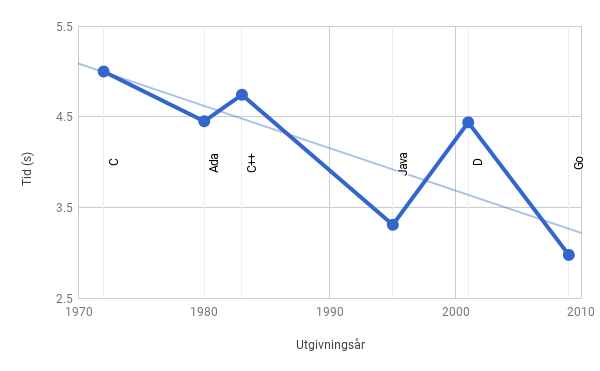
\includegraphics[width=1\textwidth,natwidth=600,natheight=371]{performance.png}
\caption{Exekveringstid över utgivningsår}
\label{figure:performance}
\end{center}
Figur \ref{figure:performance} visar ett diagram med exekveringstiden för de olika programspråken över sitt utgivningsår. Figuren visar även en trendlinje som anger riktning på exekveringstidernas utveckling över utgivningsåren.
\end{figure}

% Diagram med popularitet
\begin{figure}[H]
\begin{center}
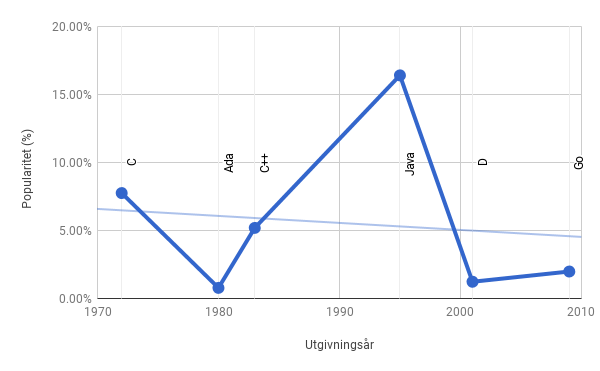
\includegraphics[width=1\textwidth,natwidth=600,natheight=371]{popularity.png}
\caption{Popularitet över utgivningsår}
\label{figure:popularity}
\end{center}
Figur \ref{figure:popularity} presenterar i tidsordning populariteten för de olika programspråken över sitt utgivningsår, på samma horisontella skala som i figur \ref{figure:performance}. Java är mest populär på strax över 16\% med utgivningsår 1995, 14 år äldre och 8 gånger mer populärt i sin användning än programspråket Go. C som är det äldsta språket i studien hade en popularitet på cirka 7.7\% och därmed det näst mest populära språket i studien.
\end{figure}


\section{Diskussion}
Om endast trendlinjen i figur \ref{figure:performance} beaktas kan en logisk följd dras att det är en fallande trend, det vill säga att exekveringstiden i programspråk blir snabbare med tiden. Ändå är det långsammaste språket C ändå det näst mest populära språket på cirka 7.7\%, jämfört med Go som var snabbast men endast hade en popularitet på ungefär 2\%. Detta kan naturligtvis bero på att C har funnits i 37 år längre än Go och därför hunnit användas till fler applikationer samt att det kanske inte lönar sig att lägga ner den tid som krävs för att skriva om program från C till Go.

I figur \ref{figure:popularity}, där programspråkens popularitet visas, blir sambanden inte lika tydliga. Att Ada och D är såpass låga på skalan skulle kunna resoneras utifrån  deras långsamma beräkningshastighet, vilket däremot motsätts med C++ som är långsammare än de båda men över dubbelt så populärt som de tidigare två tillsammans. Det mest populära programspråket är Java på strax över 16\% med utgivningsår 1995, 23 år yngre och mer än dubbelt så populärt än C som är näst mest populärt. Den höga populariteten i Java kan bero på att operativsystemet Android är byggt på samma språk vilket gör att även en stor del av apputveckling till mobiltelefoner sker i Java \citep{gruman_2017}.

Programspråk som lanseras idag har en större förväntan på sig att kunna utföra fler avancerade operationer utan att behöva skriva lång programkod \citep{stroustrup_1997}. Detta gör att kodbasen (programspråkets byggstenar) för programspråken måste innehålla mer funktioner och operationer som tynger ner programmet, men lyckas ändå verka bli snabbare med tiden \citep{luong_2017}.

Studien hade kunnat visa ett annat resultat om fler språk kunnat inkluderas. Om dessutom högnivåspråk hade inkluderats skulle dessa kunnat stärka eller motbevisa resultatet. Kompilatorn för programspråk har även en viss inverkan i hur snabbt det kompilerade programmet blir \citep{srikant_shankar_2008}, något som inte tagits hänsyn till i den här studien. Även fler typer av algoritmer skulle kunna testats för att bekräfta respektive programspråks beräkningshastighet.


\section{Slutsats}
Syftet med studien har varit att testa om beräkningshastigheten i programspråk har ett samband med hur gamla de är med hjälp av olika experiment. Trenden som visar att programspråken blir snabbare i sin beräkningshastighet med tiden skulle kunna ses som självklar då det finns mer vetskap för att utveckla programspråk idag än för 45 år sedan C först kom. Ett exempel på samma utveckling är att bilar blivit snabbare under samma tidsperiod. Programspråken har växt med fler operationer och funktioner, trots det har de inte blivit långsammare; utan tvärtom, blivit snabbare, vilket studien redovisat för.

Frågeställningen har besvarats, även om det finns fler aspekter att tillämpa för att få ett bredare resultat och ett starkare bevis på att trenden stämmer.


% Skriv ut referenser
\printbibliography

% Stäng dokumentet
\end{document}
